\chapter{Szimulációk}
A teljes struktúrát együttesen nem szimuláltam le, mivel az egyes alkotóelemek méretezését külön-külön végeztem első körben, de még nem minddel jutottam értékelhető eredményre. A differenciális vonallal és az antennával sikerült teljesítenem a követelményeket, a balun és a földkitöltés szélén az áramblokkoló mintázat még nincs használható állapotban.
\par A balun jelenlegi konstrukciójával egyszerűen nem teljesült a maximum -10 dB-s bemeneti (CPW) reflexiós követelmény a kimenet (CPS) illesztett lezárása mellett. Az áramblokkoló mintázat tervezésével pedig azért nem foglalkoztam, mert ennek a vizsgálatához érdemes a többi komponenst elfogadhatóan megtervezni, mivel ez a mintázat gyakorlatilag csak az antenna sugárzási karakterisztikáját kell, hogy befolyásolja. Ugyan a földkitöltés viselkedése az antenna bemeneti impedanciáját is kissé megváltoztathatja, de tapasztalataim szerint csak olyan mértékben, hogy az az antenna paramétereinek enyhe változtatásával az újból kihangolható.
\section{A balun transzformátor}
\par A legjobb szimulált balun bemeneti reflexió \SI{-9,2}{dB}-re adódott a teljes sávon, a szimulációhoz a balun keresztmetszetei \aref{fig:balun-kereszt}. ábrán láthatóak. A bemeneti reflexióra adódó értékekre általánosan igaz volt, hogy a vizsgált frekvenciasávban alig változott, gyakorlatilag konstans volt (\SI{0,02}{dB} eltérés a sávon belül), így a balunnak nem a sávszélessége a korlátozó tényezője.
\begin{figure}[h]
	\centering
	\begin{subfigure}[b]{0.3\textwidth}
		\centering
		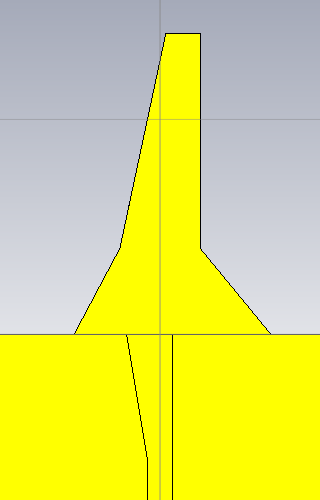
\includegraphics[width=\textwidth]{kep/results/balun_1.png}
		\caption{alsóbb rézréteg}
	\end{subfigure}
	\hfill
	\begin{subfigure}[b]{0.3\textwidth}
		\centering
		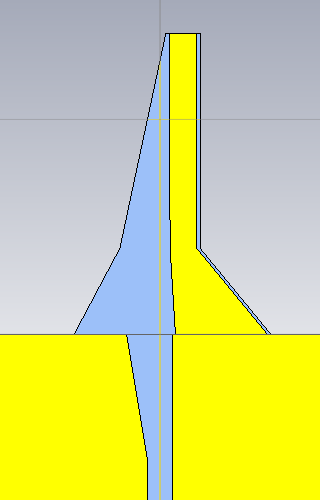
\includegraphics[width=\textwidth]{kep/results/balun_2.png}
		\caption{köztes (via) réteg}
	\end{subfigure}
	\hfill
	\begin{subfigure}[b]{0.3\textwidth}
		\centering
		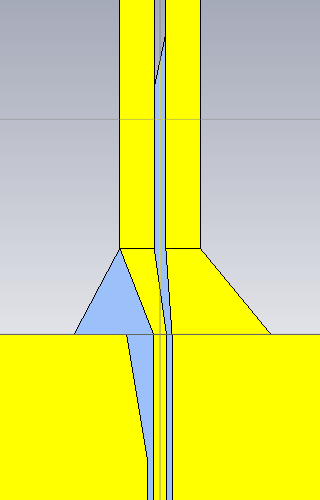
\includegraphics[width=\textwidth]{kep/results/balun_3.png}
		\caption{felső rézréteg}
	\end{subfigure}
	\caption{A szimulált balun struktúra keresztmetszetei. A sárga terület az elmetszett réz térfogat, a kék terület az alsóbb rézrétegek összesen, a szubsztrát átlátszó.}
	\label{fig:balun-kereszt}
\end{figure}
A balun szimmetrikus kimenete a szimulációk során illesztetten volt lezárva egy waveguide porttal, az így kapott \SI{-9,2}{dB}-nél feltehetően lényegesen nagyobb bemeneti reflexió is előfordulna a vizsgált sávon, ha a sávon belül változó talpponti impedanciájú antennával lenne lezárva. Emiatt valószínűleg más szerkezetű balunnal lesz érdemes próbálkozni a továbbiakban, nem pedig az eddig vizsgált struktúra méretparamétereit tovább finomhangolni. A a pontos méretparamétereket nem sorolom itt fel, mivel maga a balun a szimulációk szerint túlságosan nagy reflexiójú.
\section{Az antenna}
A három részletesebben vizsgált antennaváltozatot bemeneti reflexió, közelítő $Q$-faktor és a méretparaméterekre való érzékenység szempontjából hasonlítottam össze. Az iránykarakterisztikáik közötti különbségekkel nem foglalkoztam, mert a struktúrális hasonlóságok miatt etekintetben valószínűleg nincs közöttük számottevő különbség. A három részletesebben vizsgált változat közül végül a kiszélesedő struktúrára esett a választásom, mindkét társával szemben van valamilyen előnye, ahogy az lentebb olvasható.
\subsection{Méretekre való érzékenység}
A vizsgált antennák meglehetősen érzékenyek a méretparamétereik változtatására, de nem egyformán. A kiszélesedő szárú változat volt a leginkább érzéketlen, \SI{0,1}{mm}-nyi változás mellett a legtöbb méretparaméterében még gyakorlatilag az egész vizsgált frekvenciasávra teljesítette a \SI{-10}{dB}-nél kisebb bemeneti reflexiót. Azért éppen \SI{0,1}{mm}-es változás hatását vizsgáltam meg nagyvonalakban, mert a NYÁK gyártók kivitelezési pontossága ebbe a nagyságrendbe esik, de ennél várhatóan kisebb. Például a cégnél prototípusok gyártásánál közreműködő Eurocircuits \cite{eurocircuits} cég minimális huzalszélessége \SI{0,1}{mm}-es.
\subsection{Bemeneti reflexió}
A bemeneti reflexió szempontjából nagyon hasonlóan viselkednek ezek az antennák, ami nem meglepő, mivel a struktúrájuk hasonló és a bemeneti impedanciájukat erősen befolyásoló rövidzár hurok méretezése majdnem megegyező. Az $S_{11}$ paraméterük abszolút értéke \aref{fig:S11-dB}. ábrán látható.
\begin{figure}[h]
	\centering
	\begin{subfigure}[b]{0.7\textwidth}
		\centering
		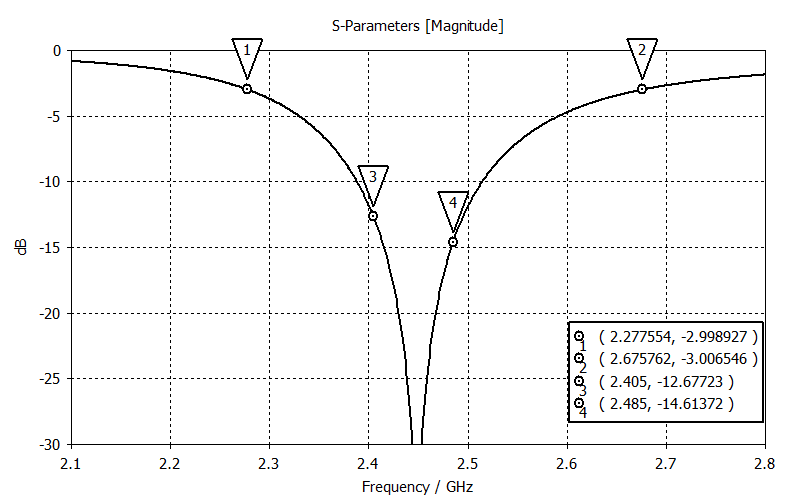
\includegraphics[width=\textwidth]{kep/results/bifa_S11_dB.png}
		\caption{egyszerű BIFA}
	\end{subfigure}
	\hfill
	\begin{subfigure}[b]{0.7\textwidth}
		\centering
		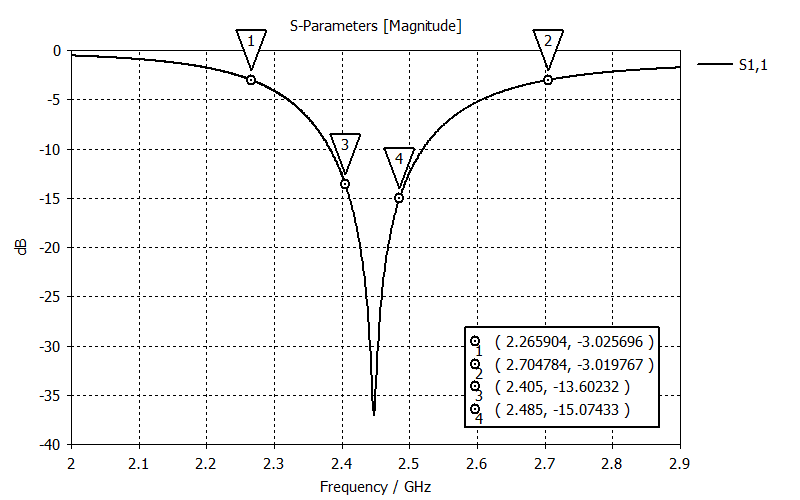
\includegraphics[width=\textwidth]{kep/results/bifa_broadband_S11_dB.png}
		\caption{kiszélesedő, visszahajló szárú BIFA}
	\end{subfigure}
	\hfill
	\begin{subfigure}[b]{0.7\textwidth}
		\centering
		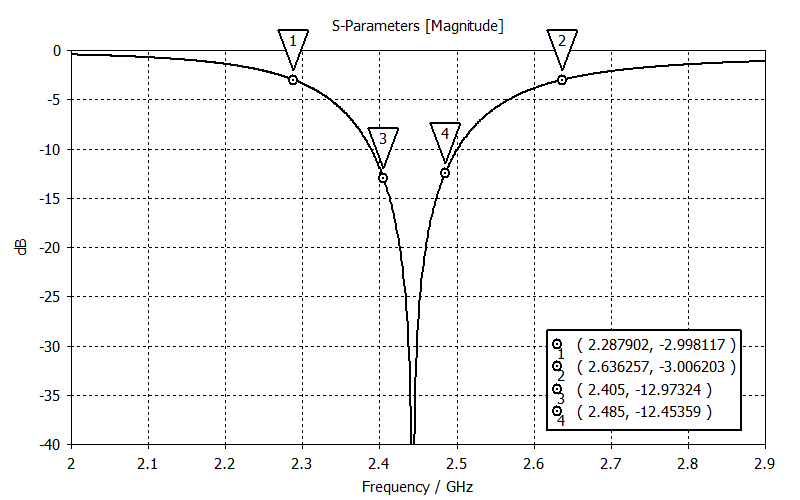
\includegraphics[width=\textwidth]{kep/results/bifa_meandered_S11_dB.png}
		\caption{menaderezett szárú BIFA}
	\end{subfigure}
	\caption{A különböző BIFA változatok $S_{11}$ paraméterei.}
	\label{fig:S11-dB}
\end{figure}
\par A három variáció közül a kiszélesedő szárú BIFA teljesített a legjobban bemeneti reflexió szempontjából, ugyan csak kevéssel. Ennek a változatnak a paraméterezése \aref{fig:bifa-bb-param}. ábrán és \aref{tab:bifa-bb-param}. táblázatban látható, az $S_{11}$ paramétere Smith-diagramon pedig \aref{fig:smith}. ábrán szerepel.
\begin{figure}[h!]
	\centering
	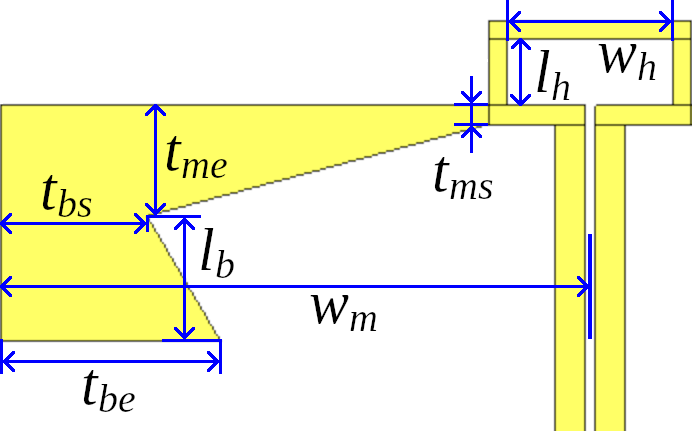
\includegraphics[width=0.5\textwidth]{kep/results/bifa_broadband_params.png}
	\caption{A kiszélesedő sárú BIFA paramétereinek értelmezése.}
	\label{fig:bifa-bb-param}
\end{figure}
\begin{table}[h!]
	\centering
	\begin{tabular}{|c|c|c|c|c|c|c|c|}
	\hline
	$w_{m}$ & $w_{h}$ & $l_{h}$ & $t_{ms}$ & $t_{me}$ & $t_{bs}$ & $t_{be}$ \\
	\hline
	\SI{16,05}{mm} & \SI{4,5}{mm} & \SI{1,8}{mm} & \SI{0,5}{mm} & \SI{3}{mm} & \SI{4}{mm} & \SI{6}{mm}\\
	\hline
	\end{tabular}
	\caption{A kiszélesedő szárú BIFA paramétereinek értékei.}
	\label{tab:bifa-bb-param}
\end{table}
\begin{figure}[h!]
	\centering
	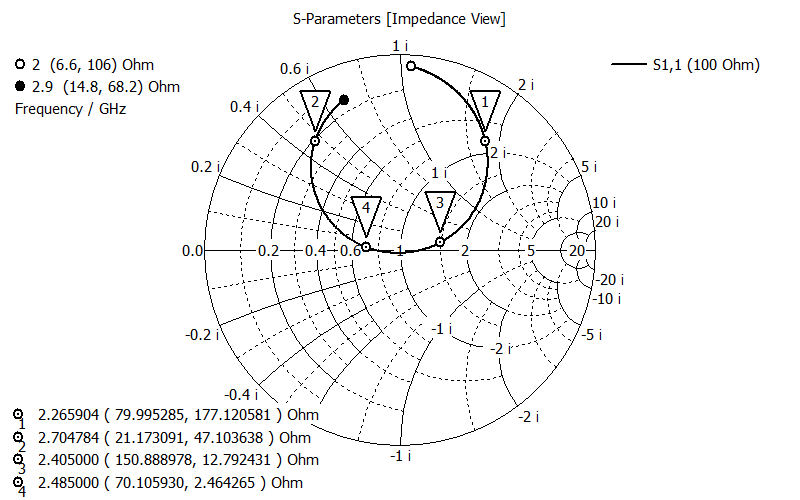
\includegraphics[width=\textwidth]{kep/results/bifa_broadband_S11_smith.png}
	\caption{A kiszélesedő szárú BIFA $S_{11}$ paramétere Smith-diagramon ábrázolva, \SI{100}{\ohm}-ra normalizálva.}
	\label{fig:smith}
\end{figure}
\subsection{$Q$-faktor}
\Aref{sec:q}. alfejezetben leírt $Q$ közelítő formulák közül a három ténylegesen alkalmazhatót kiszámítottam a három antennavariációra, a vizsgált frekvenciasáv közepére (\SI{2,45}{GHz}-re). A $Q_2$ közelítés kiszámítása rendkívül egyszerűen történt az $S_{11}$ eredmények alapján. Hasonlóan könnyen kiszámolható volt $Q_3$ is, mert CST-ben az $S_{11}$-ből rögtön származtatható a VSWR, amiből pedig már kiszámítható a $Q_3$. A legtrükkösebb a $Q_4$ meghatározása volt, mert ennél a komplex talpponti impedancia frekvencia (és nem körfrekvencia) szerinti deriváltjából kell származtatni a végeredményt. Ennek a számítási menetnek a ténylegesen használt lépései \aref{equ:actual-q4}. egyenletben láthatóak, a különböző antennákra és $Q$-kra adódó értékek pedig \aref{tab:q}. táblázatban találhatóak.
	\begin{align}
		\begin{split}\label{equ:actual-q4}
			Q_4(\omega) & = \frac{\omega}{2 R(\omega)}|Z'(\omega)| = \frac{\omega}{2 R(\omega)}\left|\frac{d Z(\omega)}{d \omega}\right| = \\[0.5ex]
						& = \frac{2 \pi f}{2 R(f)}\left|\frac{d Z(f)}{d f}\right| \frac{1}{2 \pi} = \frac{f}{2 R(f)}\left|\frac{d Z(f)}{d f}\right|
		\end{split}
	\end{align}
\begin{table}[h!]
	\centering
	\begin{tabular}{|c|c|c|c|}
	\hline
	BIFA változat 	& $Q_2$ & $Q_3$ & $Q_4$ \\
	\hline
	egyszerű 		& 60,49 & 11,11 & 12,77 \\
	\hline
	kiszélesedő 	& 56,45 & 12,05 & 12,17 \\
	\hline
	meanderezett 	& 70,00 & 14,71 & 14,52 \\
	\hline
	\end{tabular}
	\caption{Az antennaváltozatok különböző közelítő $Q$ értékei \SI{2,45}{GHz}-en.}
	\label{tab:q}
\end{table}
Nyilvánvaló, hogy a $Q_2$ közelítés kilóg a sorból, valamilyen skálázási probléma lehet a számításban vagy más $S_{11}$ határértékhez tartozó relatív sávszélességet lenne érdemes felhasználni. A három antennatípus közül a meanderezett teljesít legrosszabbul $Q$ szempontjából, a másik kettő pedig egymáshoz nagyon hasonlóan.
\begin{figure}[h!]
	\centering
	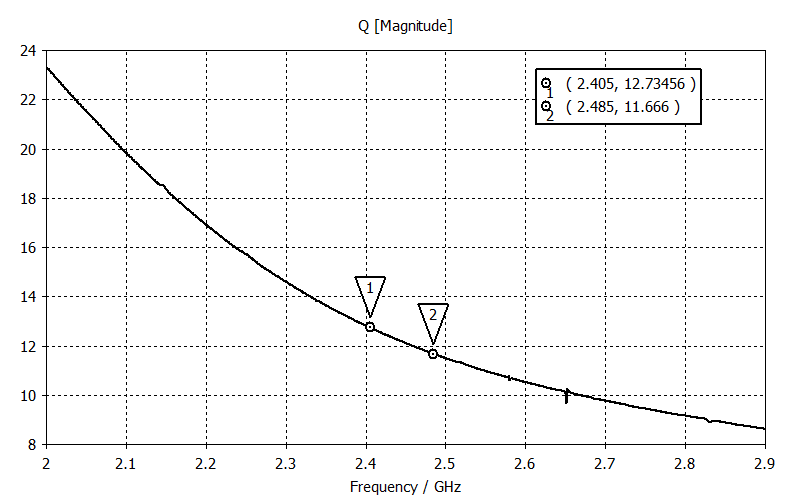
\includegraphics[width=\textwidth]{kep/results/bifa_broadband_QZ.png}
	\caption{A kiszélesedő szárú BIFA $Q_4$ paramétere.}
	\label{fig:QZ}
\end{figure}
\begin{figure}[h!]
	\centering
	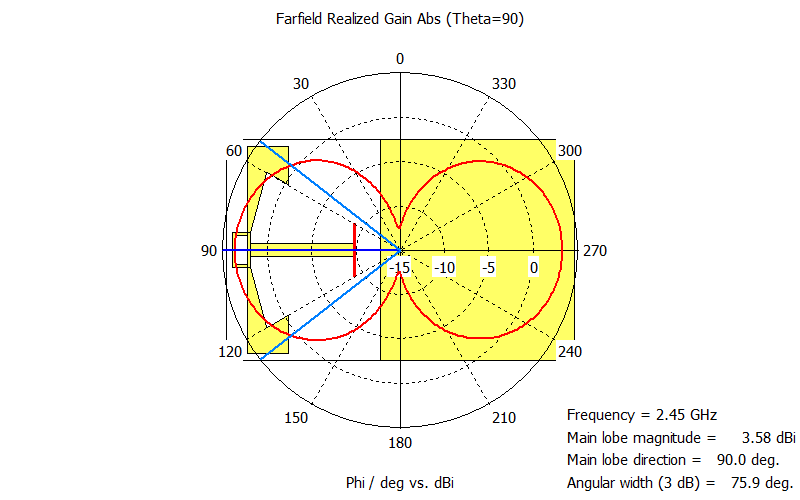
\includegraphics[width=\textwidth]{kep/results/bifa_broadband_pattern_tetha90.png}
	\caption{A kiszélesedő BIFA iránykarakterisztikájának leginformatívabb síkmetszete és ráillesztve a struktúra képe a megfelelő irányban.}
	\label{fig:pattern}
\end{figure}